% Generator: hand-authored TikZ schematic traced from the source-visible edges and labels; coordinates are illustrative only.
% Source ID: src-a2453dc34b5026e77f4d0739bc0db2e578931f651c2edf799310ddb5ccc483c4
% PDF SHA-256: ffd59c395a0c675118f6da576e48842549c4afa031d923448f26f33087bc7e85
% PDF page 1; printed page 140; question 18.
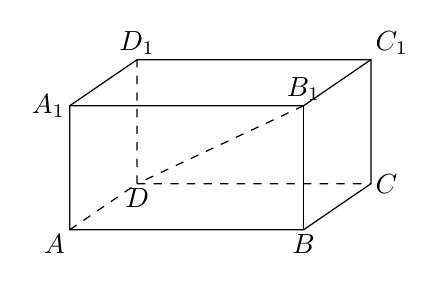
\begin{tikzpicture}[x=0.9cm,y=0.9cm,line width=0.45pt,every node/.style={inner sep=1.5pt}]
  \coordinate (A)  at (0,0);
  \coordinate (B)  at (3.3,0);
  \coordinate (C)  at (4.25,0.65);
  \coordinate (D)  at (0.95,0.65);
  \coordinate (A1) at (0,1.75);
  \coordinate (B1) at (3.3,1.75);
  \coordinate (C1) at (4.25,2.4);
  \coordinate (D1) at (0.95,2.4);

  % Visible solid edges.
  \draw (A)--(B)--(C)--(C1)--(B1)--(A1)--cycle;
  \draw (A1)--(D1)--(C1);
  \draw (B)--(B1);
  % Hidden edges and the indicated space diagonal.
  \draw[dashed] (A)--(D) (D)--(C) (D)--(D1) (B1)--(D);

  \node[below left] at (A) {$A$};
  \node[below] at (B) {$B$};
  \node[right] at (C) {$C$};
  \node[below] at (D) {$D$};
  \node[left] at (A1) {$A_1$};
  \node[above] at (B1) {$B_1$};
  \node[above right] at (C1) {$C_1$};
  \node[above] at (D1) {$D_1$};
\end{tikzpicture}
